\documentclass[tikz,border=8pt]{standalone}

\usepackage[T1]{fontenc}
\usepackage[utf8]{inputenc}
\usepackage{lmodern}
\usepackage{amsmath}
\usepackage{tikz}
\usetikzlibrary{arrows.meta,positioning,fit,calc,backgrounds}

\begin{document}
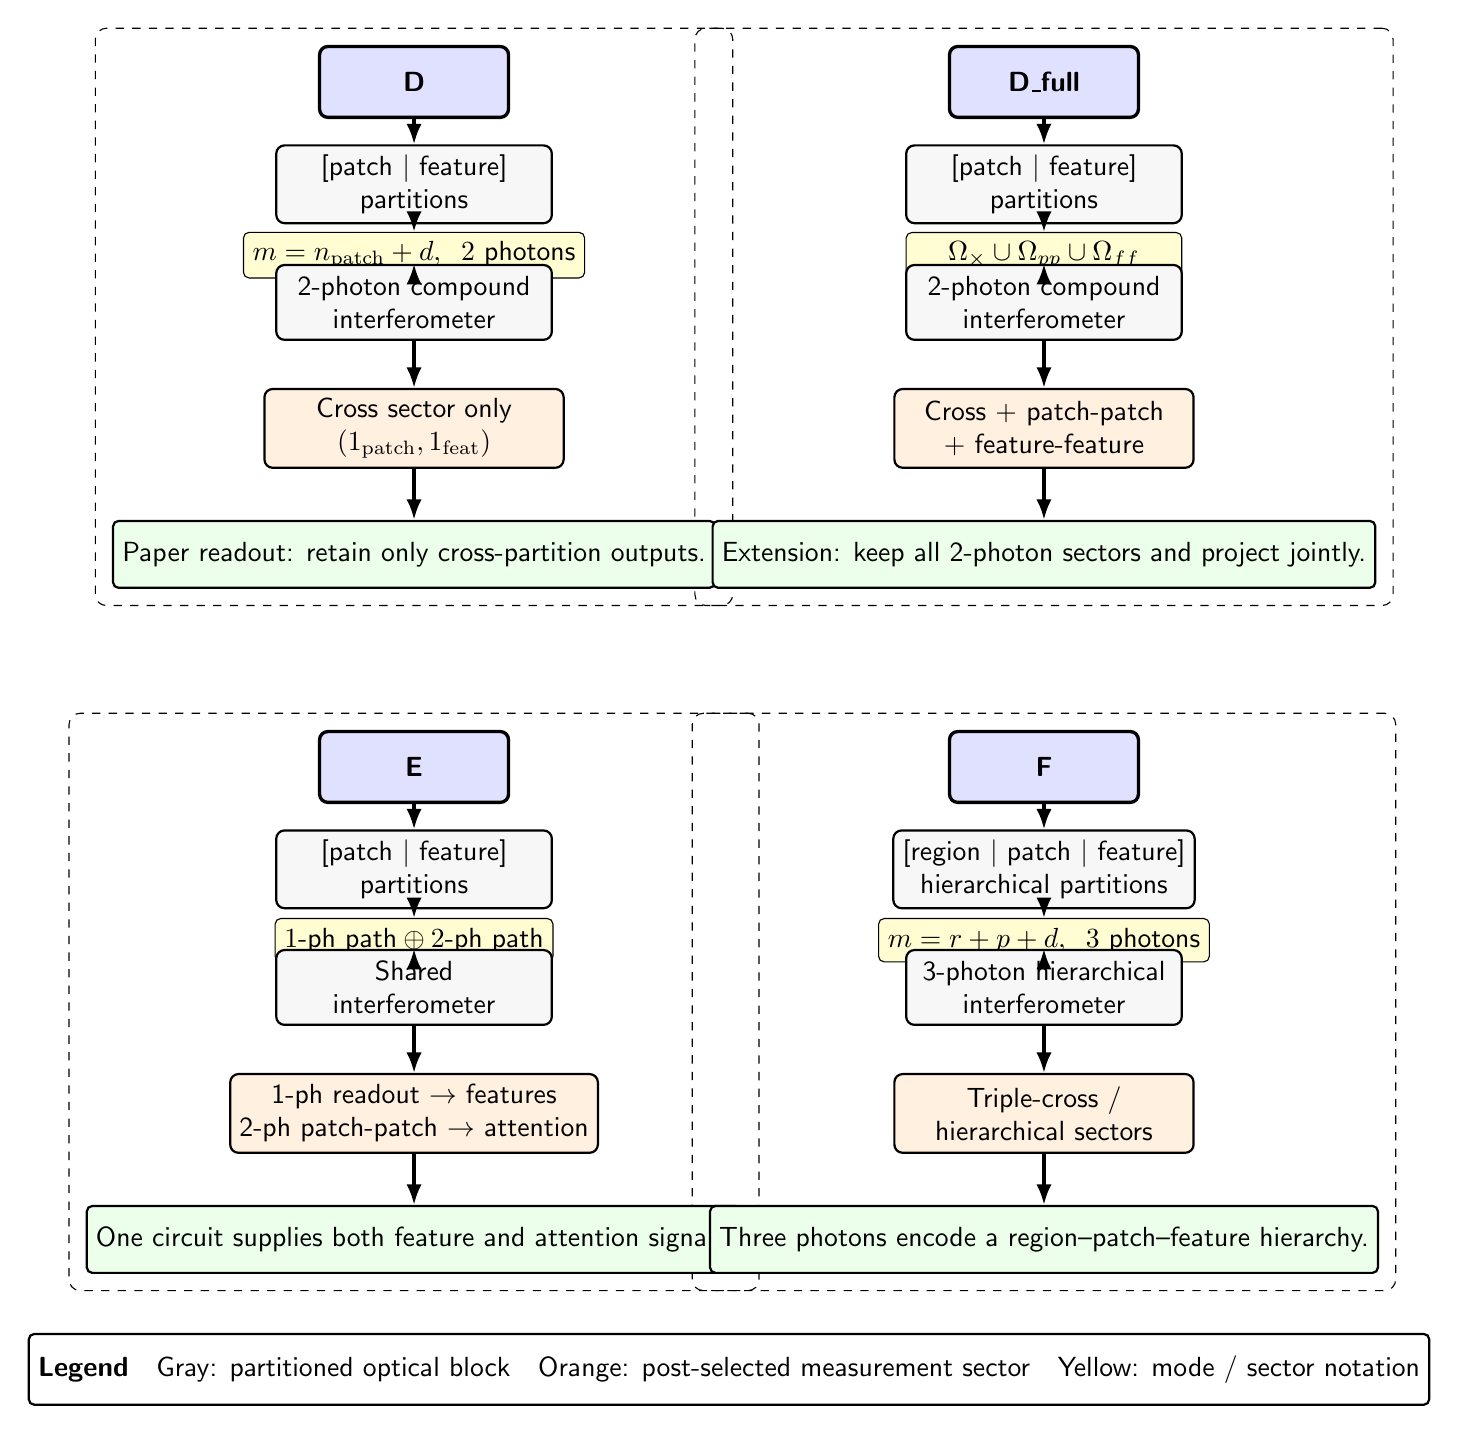
\begin{tikzpicture}[
  font=\sffamily,
  x=1cm, y=1cm,
  title/.style={draw, rounded corners=3pt, minimum width=2.4cm, minimum height=0.9cm, align=center, fill=blue!12, very thick},
  block/.style={draw, rounded corners=3pt, minimum width=3.5cm, minimum height=0.95cm, align=center, fill=gray!6, thick},
  sector/.style={draw, rounded corners=3pt, minimum width=3.8cm, minimum height=1.0cm, align=center, fill=orange!12, thick},
  ann/.style={draw, rounded corners=2pt, minimum width=3.5cm, minimum height=0.55cm, align=center, fill=yellow!18, thin},
  note/.style={draw, rounded corners=2pt, minimum width=4.2cm, minimum height=0.85cm, align=center, fill=green!8, thick},
  legend/.style={draw, rounded corners=2pt, minimum width=7.6cm, minimum height=0.9cm, align=left, fill=white, thick},
  arrow/.style={-{Latex[length=2.6mm]}, very thick},
  dashedbox/.style={draw, dashed, rounded corners=4pt, inner sep=6pt}
]

\node[title]  (d)   at (3.2, 0.0) {\textbf{D}};
\node[block]  (d1)  at (3.2, -1.3) {[patch $\mid$ feature]\\partitions};
\node[ann]  (ds1) at (3.2, -2.2) {$m = n_{\mathrm{patch}} + d,\;\; 2 \text{ photons}$};
\node[block]  (d2)  at (3.2, -2.8) {2-photon compound\\interferometer};
\node[sector] (d3)  at (3.2, -4.4) {Cross sector only\\$(1_{\mathrm{patch}},1_{\mathrm{feat}})$};
\node[note]   (d4)  at (3.2, -6.0) {Paper readout: retain only cross-partition outputs.};

\node[title]  (df)  at (11.2, 0.0) {\textbf{D\_full}};
\node[block]  (df1) at (11.2, -1.3) {[patch $\mid$ feature]\\partitions};
\node[ann]  (dfs1) at (11.2, -2.2) {$\Omega_{\times} \cup \Omega_{pp} \cup \Omega_{ff}$};
\node[block]  (df2) at (11.2, -2.8) {2-photon compound\\interferometer};
\node[sector] (df3) at (11.2, -4.4) {Cross + patch-patch\\+ feature-feature};
\node[note]   (df4) at (11.2, -6.0) {Extension: keep all 2-photon sectors and project jointly.};

\node[title]  (e)   at (3.2, -8.7) {\textbf{E}};
\node[block]  (e1)  at (3.2, -10.0) {[patch $\mid$ feature]\\partitions};
\node[ann]  (es1) at (3.2, -10.9) {$1\text{-ph path} \oplus 2\text{-ph path}$};
\node[block]  (e2)  at (3.2, -11.5) {Shared\\interferometer};
\node[sector] (e3)  at (3.2, -13.1) {1-ph readout $\rightarrow$ features\\2-ph patch-patch $\rightarrow$ attention};
\node[note]   (e4)  at (3.2, -14.7) {One circuit supplies both feature and attention signals.};

\node[title]  (f)   at (11.2, -8.7) {\textbf{F}};
\node[block]  (f1)  at (11.2, -10.0) {[region $\mid$ patch $\mid$ feature]\\hierarchical partitions};
\node[ann]  (fs1) at (11.2, -10.9) {$m = r + p + d,\;\; 3 \text{ photons}$};
\node[block]  (f2)  at (11.2, -11.5) {3-photon hierarchical\\interferometer};
\node[sector] (f3)  at (11.2, -13.1) {Triple-cross /\\hierarchical sectors};
\node[note]   (f4)  at (11.2, -14.7) {Three photons encode a region--patch--feature hierarchy.};

\node[legend] (leg) at (7.2, -16.35) {\textbf{Legend}\quad Gray: partitioned optical block\quad Orange: post-selected measurement sector\quad Yellow: mode / sector notation};

\draw[arrow] (d.south) -- (d1.north);
\draw[arrow] (d1.south) -- (ds1.north);
\draw[arrow] (ds1.south) -- (d2.north);
\draw[arrow] (d2.south) -- (d3.north);
\draw[arrow] (d3.south) -- (d4.north);

\draw[arrow] (df.south) -- (df1.north);
\draw[arrow] (df1.south) -- (dfs1.north);
\draw[arrow] (dfs1.south) -- (df2.north);
\draw[arrow] (df2.south) -- (df3.north);
\draw[arrow] (df3.south) -- (df4.north);

\draw[arrow] (e.south) -- (e1.north);
\draw[arrow] (e1.south) -- (es1.north);
\draw[arrow] (es1.south) -- (e2.north);
\draw[arrow] (e2.south) -- (e3.north);
\draw[arrow] (e3.south) -- (e4.north);

\draw[arrow] (f.south) -- (f1.north);
\draw[arrow] (f1.south) -- (fs1.north);
\draw[arrow] (fs1.south) -- (f2.north);
\draw[arrow] (f2.south) -- (f3.north);
\draw[arrow] (f3.south) -- (f4.north);

\begin{scope}[on background layer]
  \node[dashedbox, fit=(d) (d4)] {};
  \node[dashedbox, fit=(df) (df4)] {};
  \node[dashedbox, fit=(e) (e4)] {};
  \node[dashedbox, fit=(f) (f4)] {};
\end{scope}
\end{tikzpicture}
\end{document}
